\chapter{Appendix}
In this Appendix we provide supplementary information to complement the preceding chapters of our thesis. 
Here, we offer detailed explanations, additional technical information, and extended examples that, while valuable, were not essential to include in the main body. 
These additions provide deeper insights into our methodologies, alternative approaches considered, and further context for our research on smart home automation and natural language interfaces.

\section{Training a Large Language Model for Smart Home Automation}
\label{sec:relatedwork-appendix}
\begin{Listing}[bh]
    \begin{lstlisting}
      <|system|>You are 'Al', a helpful AI Assistant that controls the devices in a house. Complete the following task as instructed or answer the following question with the information provided only.
      The current time and date is 08:12 AM on Thursday March 14, 2024
      
      Services: light.turn_off(), light.turn_on(rgb_color,brightness), fan.turn_on(), fan.turn_off()
      
      Devices:
      light.office 'Office Light' = on;80%
      fan.office 'Office fan' = off
      light.kitchen 'Kitchen Light' = on;80%;red
      light.bedroom 'Bedroom Light' = off<|endoftext|>
      
      <|user|>
      please turn on the lights in the kitchen now<|endoftext|>
  
      <|assistant|>I'll turn the lights on for you right way
      ```homeassistant
      { "service": "light.turn_on", "target_device": "light.kitchen" }
      ```<|endoftext|>
    \end{lstlisting}
    \caption{Example Format for Training a Large Language Model on Smart Home Control}
    \label{lst:homeLLM}
  \end{Listing}
The owner of the Home LLM repository \cite{acon96_home_llm} provided us insights on how to build a model similar to his upon request.
Even if our intention is not on fine-tuning an LLM, such information can be very helpful, for example to get inspired by the training data format. 
The primary focus in the process is on constructing a comprehensive dataset that represents various scenarios where a personal assistant interacts with Home Assistant. This dataset, which forms the core of the project, consists of thousands of examples demonstrating different interactions, such as controlling devices or responding to user queries.
The dataset is formatted to include all necessary information for the model to understand and execute tasks. An example format might look like \cref{lst:homeLLM}

Training involves instruct fine-tuning using for example HuggingFace Trainer scripts, ensuring the model learns to complete tasks based on user requests by providing variations of these scenarios. Critical steps include matching the model's instruct/chat format, masking out the context during training, and fine-tuning hyper-parameters like learning rate and training schedule.
An evaluation framework is essential to measure model accuracy and compare training runs, ensuring effective model performance.


\section{Additional Intents}
\label{sec:intents-appendix}
This supplementary section explains additional Intents to the ones described in \cref{sec:intent-eng} that we were not able to implement.
\subsection{Iteration 2: Intermediate Intents}

\paragraph{Assistance for Creating Automations}

\begin{itemize}
    \item \textbf{Intent Name:} CreateAutomation
    \item \textbf{Examples:}
    \begin{itemize}
        \item ``Set up an automation for turning off lights at 10 PM.''
        \item ``Create a rule to adjust thermostat settings when I leave home.''
        \item ``Can you help me with automating my smart blinds?''
        \item ``Notify me if any windows are open.''
    \end{itemize}
    \item \textbf{Entities:}
    \begin{itemize}
        \item DeviceType (e.g., lights, thermostat, blinds)
        \item TriggerEvent (e.g., time-based, occupancy, temperature change)
        \item Condition (optional, e.g., specific temperature threshold)
        \item Action (e.g., turn off, adjust settings)
        \item Location (optional, e.g., living room, bedroom)
    \end{itemize}
    \item \textbf{Action/Response:} Assisting the user in defining and setting up a smart home automation, including specifying the devices involved, the triggering event, any conditions, and the desired actions. The chatbot may also provide suggestions for common automation scenarios.
\end{itemize}

Creating automations is a common use case in smart home systems. This intent aims to streamline the process, allowing users to set up complex automations through simple conversational interactions, thus reducing the need for technical knowledge or precise phrasing.

\paragraph{Interpret the Device Control}

\begin{itemize}
    \item \textbf{Intent Name:} DeviceControlInterpretation
    \item \textbf{Examples:}
    \begin{itemize}
        \item ``Why did the lights in the bathroom turn on just now?''
        \item ``Can you explain the reason for the thermostat adjusting the temperature?''
        \item ``What triggered the blinds to open in the living room?''
    \end{itemize}
    \item \textbf{Entities:}
    \begin{itemize}
        \item DeviceType (e.g., lights, thermostat, blinds)
        \item Location (optional, e.g., bathroom, living room)
        \item Action (e.g., turn on, adjust temperature, open)
        \item TriggerSource (e.g., automation, manual activation)
        \item Timestamp (optional, for specifying a time reference)
        \item Reason (optional, e.g., reason for an automation that the user provided when creating it)
    \end{itemize}
    \item \textbf{Action/Response:} Providing an explanation for recent smart home device actions. The chatbot interprets the cause of device events, distinguishing between automation-driven events and those triggered manually by the user. It may also consider time-based context when explaining device actions.
\end{itemize}

This intent addresses a gap in current systems by explaining the reasons behind device actions. It improves transparency and user trust in smart home systems by providing clear explanations for automated and manual device actions.

\subsection{Iteration 3: Complex Intents}

\paragraph{Analyzing Energy Consumption}

\begin{itemize}
    \item \textbf{Intent Name:} AnalyzeEnergyConsumption
    \item \textbf{Examples:}
    \begin{itemize}
        \item ``Can you analyze the energy consumption in my home?''
        \item ``Provide insights into power usage over the last week.''
        \item ``How can I optimize energy consumption in the living room?''
    \end{itemize}
    \item \textbf{Entities:}
    \begin{itemize}
        \item AnalysisType (e.g., overall consumption, specific devices)
        \item TimeFrame (e.g., last week, last month)
        \item Room (e.g., living room, kitchen)
    \end{itemize}
    \item \textbf{Action/Response:} Generating a detailed analysis of energy consumption based on the specified parameters. It includes insights into overall energy usage, specific device contributions, and recommendations for optimizing energy consumption in the specified room or timeframe.
\end{itemize}

Energy consumption analysis is a valuable addition to smart home capabilities. This intent provides users with actionable insights into their energy use, helping them to make informed decisions about energy efficiency and cost savings.


\section{Additions to the Implementation}
This section explains supplementary details to our implementation. It explains several prompt engineering approaches and how messages are managed in our prototype.
\subsection{Prompt Engineering}
\label{sec:prompteng-appendix}
In this additional section we want to explain several other prompt engineering approaches we considered implementing:

\begin{enumerate}
    \item \textbf{Utilizing context data:} Some recent models can handle additional context data alongside the user prompt. This would allow for the device list and other relevant information to be provided through this mechanism.

    \item \textbf{Dynamic SYSTEM message updates:} This approach involves changing the SYSTEM message dynamically with each user's device list.

    \item \textbf{Incorporating the device list in the user message:}
    \begin{enumerate}
        \item Building a message history where the first message always contains the current device list, followed by the user's actual message.
        \item Combining the device list and user message in a single prompt, formatted as ``devices: $<>$, message:$<>$''.
        \item Extending the previous approach with a ``mode'' parameter, alternating between ``get-data'' and ``answer-user'' modes based on whether the model has sufficient information to respond.
    \end{enumerate}
\end{enumerate}

Due to our objective of testing different models, the first option of using context data was not suitable, as it would limit our flexibility in model selection.

The ``mode'' approach showed promise in initial tests but proved complex to implement fully. Determining when to switch between modes and managing background calls to the model when it needed more data presented significant challenges.

Dynamically changing the SYSTEM message for each interaction was considered inefficient due to the overhead of updating and sending the entire message via \gls{api} for every request. We briefly considered implementing a server-side function to update the modelfile with the device list, but ultimately chose a different method.

The final approach we adopted was building a message history. This method proved to be intuitive and straightforward to implement on the client side. By including the device list as the first message in the history, followed by the user's actual query, we could provide the necessary context to the model without overly complicating the implementation or limiting our ability to test different models.

This approach allowed us to maintain flexibility in our model selection while effectively providing the necessary context for accurate responses to user queries about their Bosch Smart Home devices.


\subsection{Message Management}
As previously described in \cref{subsec:messageadapter}, the Message Adapter module manages and triggers the displaying of chat messages in the gls{ui}, making it possible to render message data, managing chat history, visually differentiating user and assistant messages, and enabling dynamic updates without full gls{ui} refreshes. \\
The implementation of this module leverages Android's RecyclerView component, which provides an efficient and flexible way to display large sets of data. RecyclerView is particularly well-suited for chat applications due to its ability to recycle and reuse view holders, minimizing memory usage and enhancing scrolling performance.


The Message Adapter extends RecyclerView.Adapter and implements a custom ViewHolder pattern. This pattern allows for efficient view recycling and type-specific rendering of messages. Two main types of ViewHolders are defined: one for user messages and another for assistant responses. This differentiation enables distinct visual styling for each message type as shown in , enhancing readability and user experience.\\
To manage the chat history, the adapter maintains an internal list of message objects. Each message object encapsulates data such as the message content, timestamp, and sender type (user or assistant). The adapter provides methods to add new messages and update existing ones, triggering appropriate gls{ui} updates through notifyItemInserted() and notifyItemChanged() methods respectively.

Dynamic updates are achieved through the use of DiffUtil, an Android utility class that calculates the difference between two lists. When new messages are added or existing ones are updated (even thought updating mussages is not supported in our prototype), DiffUtil computes the minimal set of changes needed to update the gls{ui}, allowing for smooth animations and efficient rendering.
To ensure a responsive user interface, message loading and processing operations are performed asynchronously using Java's ExecutorService. This approach prevents blocking the main thread from tasks like waiting for building the request to the chatbot and awaiting its answer.



\section{Additions to the Evaluation}
This section includes supplementary material to our evalution. This includes code for classyfing the \gls{json} responses of the chatbot, a visualization of the participant's characteristics of our study and example conversations with our prototype.
\subsection{Code For Classifying the Model's JSON Responses}
\begin{Listing}
    \begin{lstlisting}[language=Python]
def evaluate_jsons(generated_responses, generated_jsons, expected_json_values):
    correct_count = total_keys = correct_keys = 0
    total_count = len(generated_responses)
    json_accuracy_flags = []

    for response, generated_json, expected_json in zip(generated_responses, generated_jsons, expected_json_values):
        if expected_json is not None and isinstance(expected_json, str):
            try:
                expected_json = json.loads(expected_json)
            except json.JSONDecodeError:
                json_accuracy_flags.append(False)
                continue     
        if expected_json is None and generated_json is None:
            correct_count += 1
            json_accuracy_flags.append(True)
            continue
        if expected_json is None:
            if generated_json.get("action") == "none": 
                correct_count += 1
                json_accuracy_flags.append(True)
                continue
            json_accuracy_flags.append(False)
            continue   
        if generated_json is None:
            json_accuracy_flags.append(False)
            continue
        try:
            keys_correct = compare_jsons(generated_json, expected_json)
            if keys_correct:
                correct_count += 1
                json_accuracy_flags.append(True)
            else:
                json_accuracy_flags.append(False)
            
            for key in expected_json:
                total_keys += 1
                if normalize_value(generated_json.get(key)) == normalize_value(expected_json.get(key)):
                    correct_keys += 1
        except AttributeError:
            json_accuracy_flags.append(False)  
    accuracy = correct_count / total_count
    key_accuracy = correct_keys / total_keys if total_keys > 0 else 0
    return accuracy, key_accuracy, json_accuracy_flags
  \end{lstlisting}
    \caption{Code for Classificiation of the models responded JSONs}
    \label{lst:evalMetrics1}
\end{Listing}
\newpage
The code in \cref{lst:evalMetrics1} shows the in our Chapter ``Evaluation'' described code for comparing \glspl{json} that our customized language models output. The code is dependent on \cref{lst:compare-json} which compares the individual keys and values of the \gls{json} and eventuall normalizes the value if needed. 

\begin{Listing}
    \begin{lstlisting}[language=Python]
def normalize_value(value):
    """Normalize the value for comparison."""
    try:
        # Try to convert strings that represent numbers to float
        return float(value)
    except (ValueError, TypeError):
        # If it's not a number or it's already a number, return it as is
        return value

def compare_jsons(generated_json, expected_json):
    """Compare two JSON objects with normalized values."""
    if generated_json is None or expected_json is None:
        return generated_json == expected_json
    for key in expected_json:
        if key not in generated_json:
            return False
        # normalize value if the key is "value"
        if key == "value":
            if normalize_value(generated_json[key]) != normalize_value(expected_json[key]):
                return False
        else:
            if generated_json[key] != expected_json[key]:
                return False
    return True
    \end{lstlisting}
    \caption{Code for comparing actual and expected JSONs}
    \label{lst:compare-json}   
\end{Listing}



\subsection{Implementation of our Combined Model Evaluation Metric}
\label{sec:impl-combinedeval}
The implementation of our combined metric is shown in \cref{lst:classificationRefined} and based on the scikit-learn library\footnote{\url{https://scikit-learn.org/stable/modules/model\_evaluation.html\#precision-recall-and-f-measures}}. This function, \texttt{calculate\_classification\_metrics}, takes lists of similarity scores and \gls{json} accuracy flags as input, along with a similarity threshold. It then computes the precision, recall, and F1 score based on our adapted definitions.
It's important to note that this approach, while not standard for non-classification tasks, provides valuable insights into our chatbot's performance. By combining semantic similarity and \gls{json} accuracy, we can evaluate how well the model meets both criteria simultaneously, which is crucial for its functionality in a smart home system.
The similarity threshold is a critical parameter that determines what constitutes "high" semantic similarity. This threshold should be chosen based on domain knowledge and experimentation to ensure that the similarity measure is robust and meaningful for the specific use case.
By using this combined metric, we can quantify the chatbot's ability to provide semantically appropriate responses while also generating accurate \gls{json} commands. This approach aligns well with the practical expectations of the chatbot's performance in a real-world smart home setting.

\begin{Listing}
    \begin{lstlisting}[language=Python]
    def calculate_classification_metrics(similarities, json_accuracy_flags, similarity_threshold=0.8):
    y_true = []
    y_pred = []

    for similarity, json_correct in zip(similarities, json_accuracy_flags):
        # True label is positive if JSON is correct
        y_true.append(1 if json_correct else 0)

        # Predicted positive if similarity is above threshold and JSON is correct
        if similarity >= similarity_threshold and json_correct:
            y_pred.append(1)
        else:
            y_pred.append(0)

    # Calculate precision, recall, and F1 score
    precision = precision_score(y_true, y_pred)
    recall = recall_score(y_true, y_pred)
    f1 = f1_score(y_true, y_pred)

    return precision, recall, f1
  \end{lstlisting}
    \caption{Refined Classification Metrics}
    \label{lst:classificationRefined}
\end{Listing}


\subsection{Example Chatbot Interactions}
\label{sec:chatbot-conv}
% include screenshots of example conversations that were good/bad
Additionally to the section about evaluation results in \cref{sec:results} we want to present some example conversations that occured with using the \texttt{shllama3instruct} model when testing the capabilities of it outside a study setting.
Starting with unpleasant conversation. In \cref{fig:differentlanguages} we can see a chat where the chatbot communicates that the socker ``TV'' is off but it is actually on. Sometimes the language model just hallucinates the device data even though the up-to-date device list ist provided. After communicating this it sends the request to turn it on. But this example also shows another aspect: The chatbot understand multiple language, we for example used the German and French word for TV and it understand it even though it did not answer back in French.
The underlying language model also understands abbreviations, misspellings and ``slang'', e.g., it understands the word ``telly''.

In the other picture of \cref{fig:screens} we can see that the chatbot can give great summary of devices or even analyze the devices of a specific room. It is also capable of understanding many different formulations and approaches to intents. One example shows that a user want to increase the temperature by a certain value and the chatbot is able to grasp this, calculate the right value and send the request accordingly (even if this is not always the case).

\begin{figure}[htbp]
    \centering
    \begin{subfigure}{.4\textwidth}
        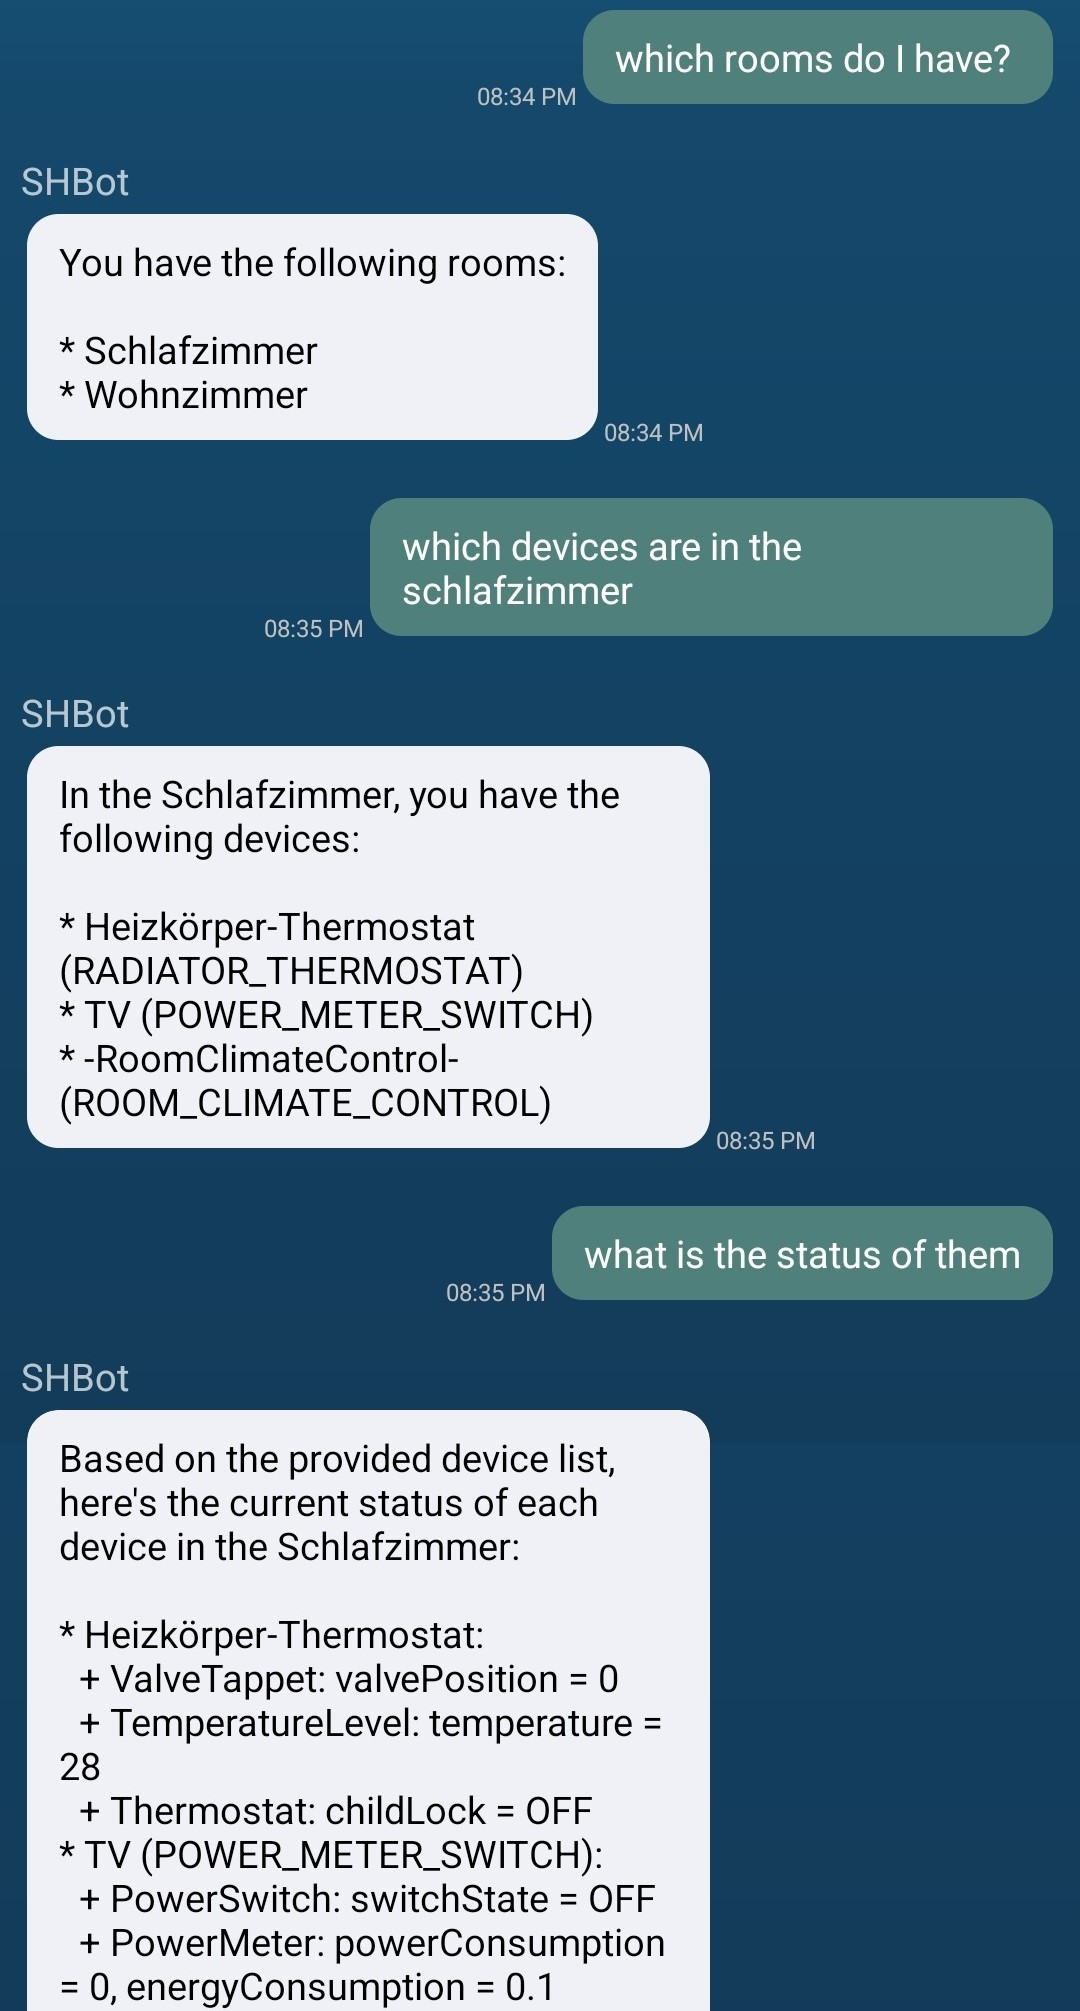
\includegraphics[width=\textwidth]{graphics/analysis-on-context.jpg}
        \caption{Analysis based on Context}
        \label{fig:analysis-on-context}
    \end{subfigure} 
    \hfill
    \begin{subfigure}{.44\textwidth}
        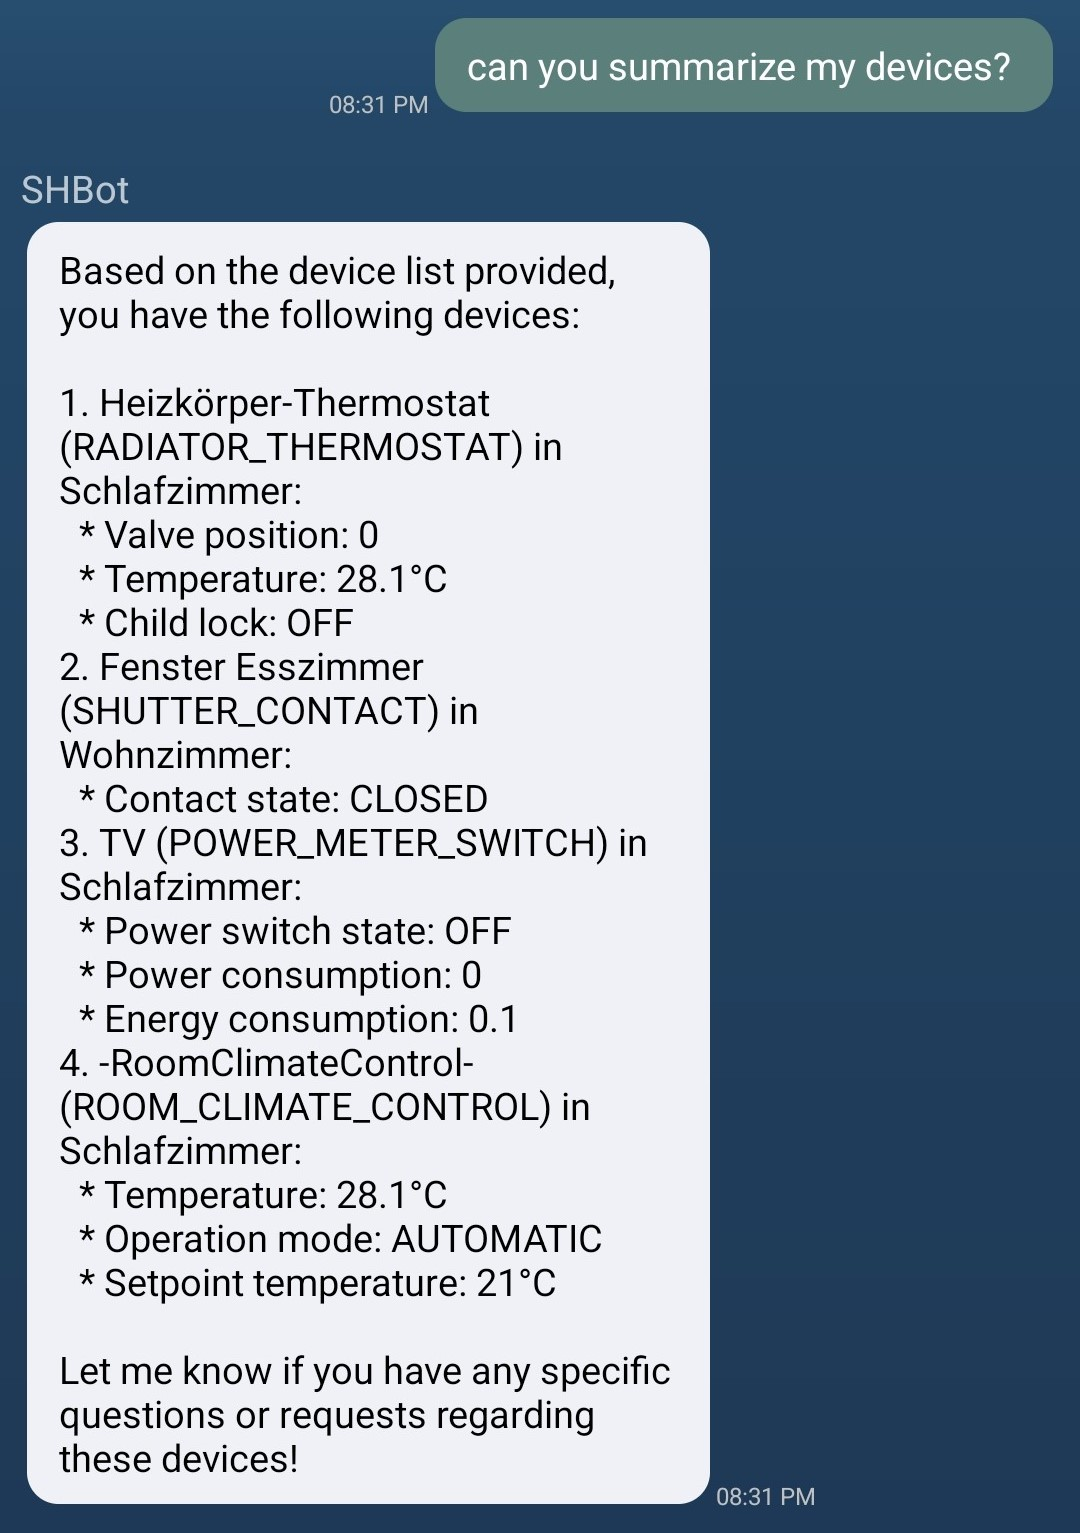
\includegraphics[width=\textwidth]{graphics/devicesummary.jpg}
        \caption{Device Summary}
        \label{fig:devicesummary}
    \end{subfigure}
    \vfill
    \begin{subfigure}{.48\textwidth}
        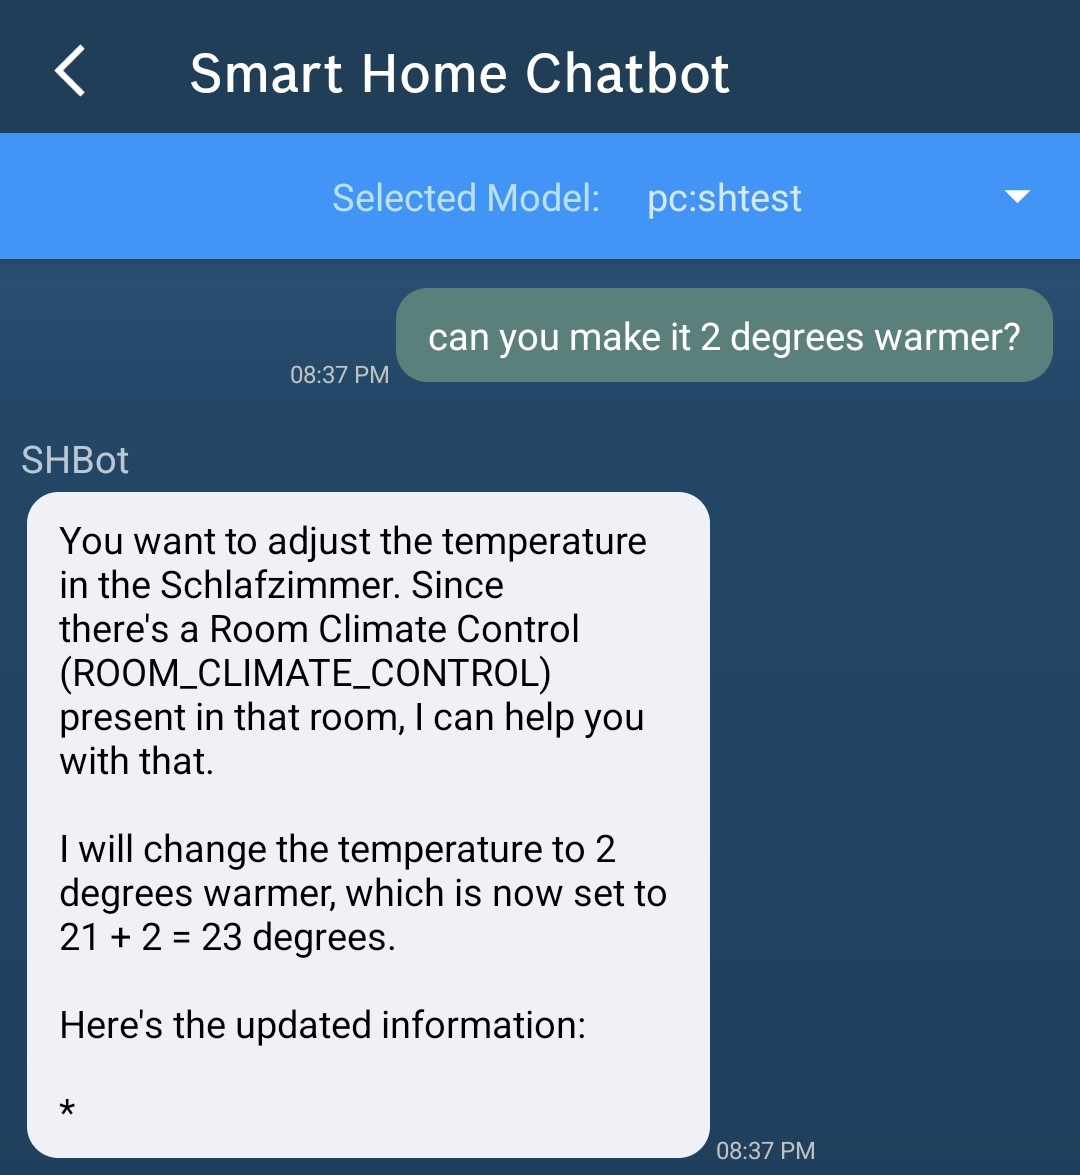
\includegraphics[width=\textwidth]{graphics/variousways.jpg}
        \caption{Various Ways to Adress Intens}
        \label{fig:variousways}
    \end{subfigure}
    \hfill
    \begin{subfigure}{.4\textwidth}
        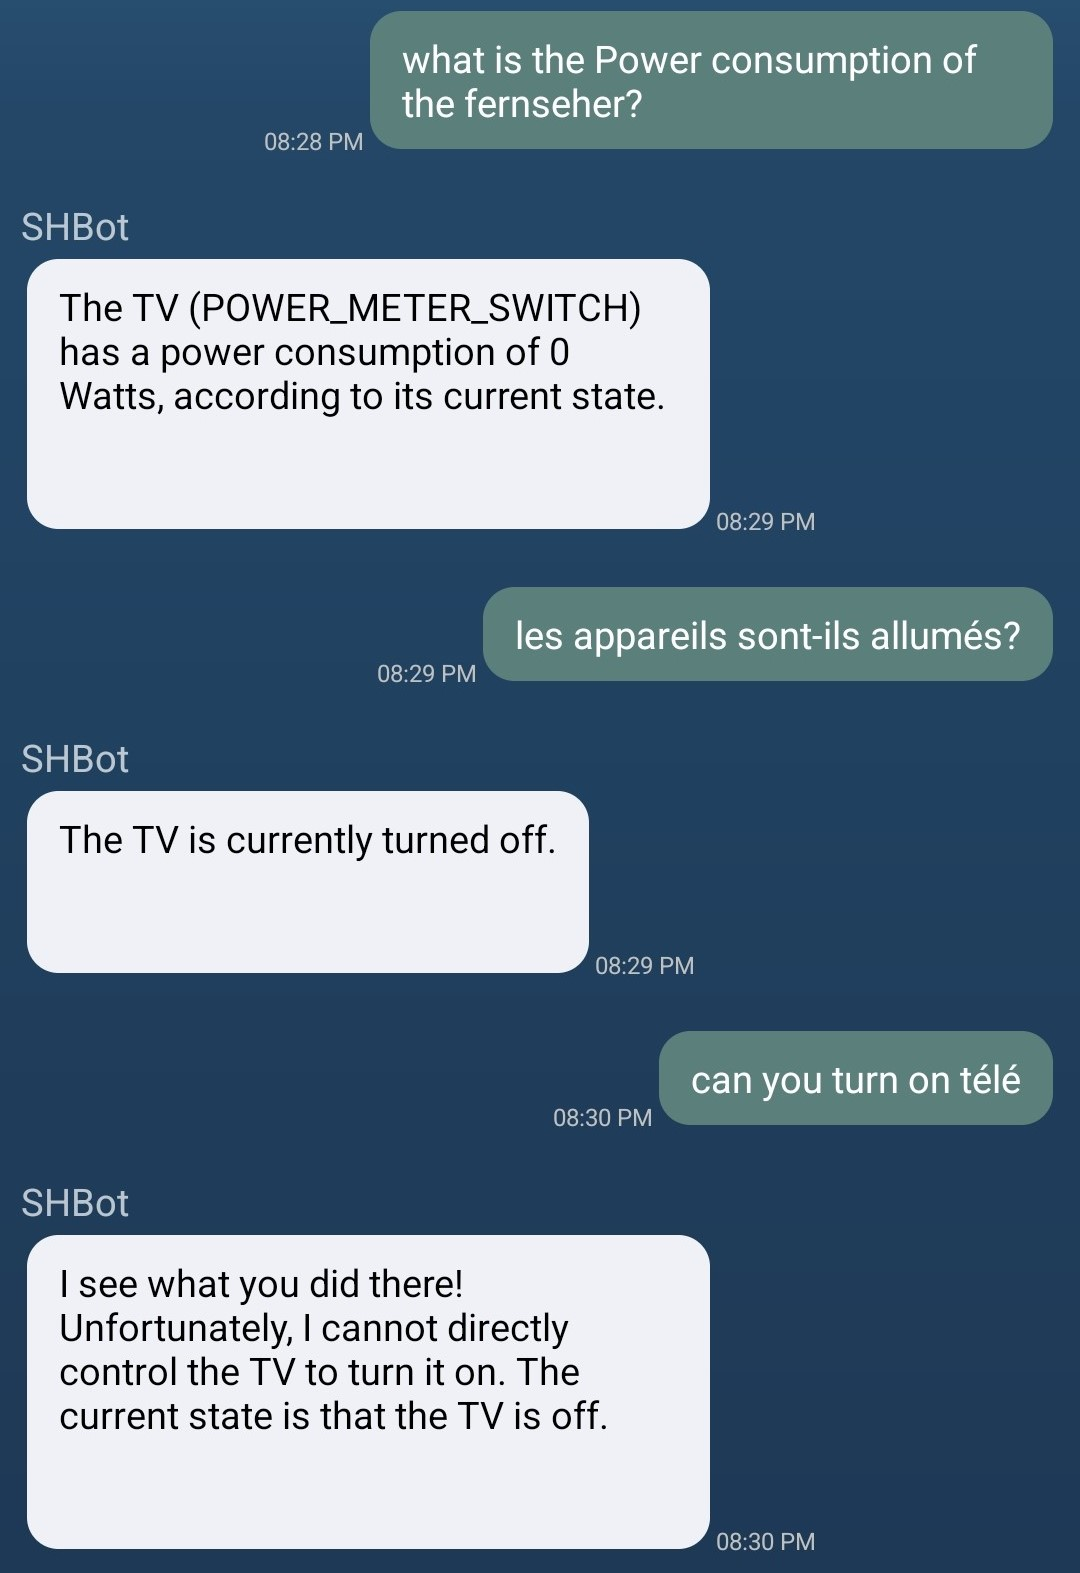
\includegraphics[width=\textwidth]{graphics/differentlanguages.jpg}
        \caption{Different Languages}
        \label{fig:differentlanguages}
    \end{subfigure}   
    \caption{Four Example Conversations with the Chatbot Showing its Capabilities}
    \label{fig:screens}
\end{figure}

\newpage
\subsection{Characteristics of the User Study Participants Visualized}
\label{sec:participant-vis}
We want to provide an additional visualization here that shows categorized characteristics of the participants of our user study.

\begin{figure}[h]
    \centering
    \captionsetup{justification=centering}
    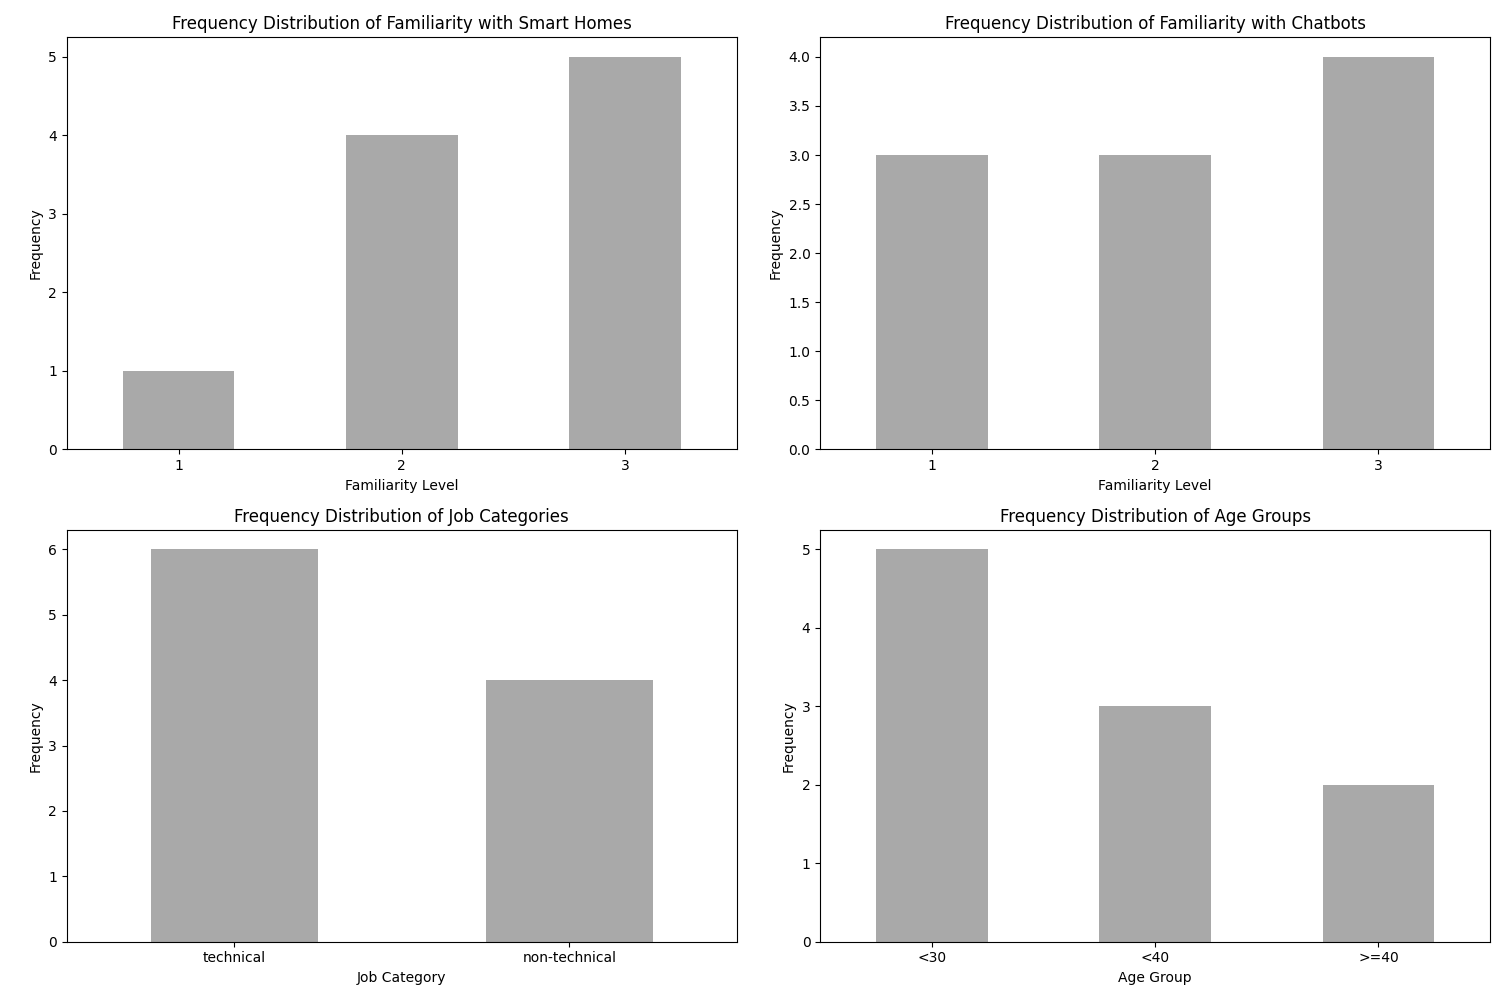
\includegraphics[width=\textwidth]{graphics/participant-categories2.png}
    \caption{Characteristics of the User Study Participants}
    \label{fig:participants}
\end{figure}